\mode*

\section{Disposition}

\begin{frame}
  \begin{figure}
    
\includegraphics[height=0.8\textheight]{fig/book.jpg}
    \caption{Front cover of Necessary Conditions of Learning.}
  \end{figure}
\end{frame}

\begin{frame}
  \begin{enumerate}
    \item What makes humans human?
    \item What is to be learned?
    \alert{\item Sameness and difference in learning}
    \item What does the world look like to others?
    \item The art of learning
    \item Making learning possible
    \item Learning to help others to learn
  \end{enumerate}
\end{frame}

\begin{frame}
  \begin{block}{Ch 3 Sameness and difference in learning}
    \begin{itemize}
      \item The problem with direct reference (induction).
      \item The patterns: contrast, generalization, fusion.
      \item \textcquote[p.~71]{NecessaryConditionsOfLearning}{%
          \textins{P}racticing something other than what was tested was more 
          effective than practicing exactly what was tested.%
        }
    \end{itemize}
  \end{block}
\end{frame}

\section{Variation theory}

\subsection{An experiment}

\begin{frame}\label<2>{vtind}
  \begin{figure}
  \begin{subfigure}{0.2\columnwidth}
    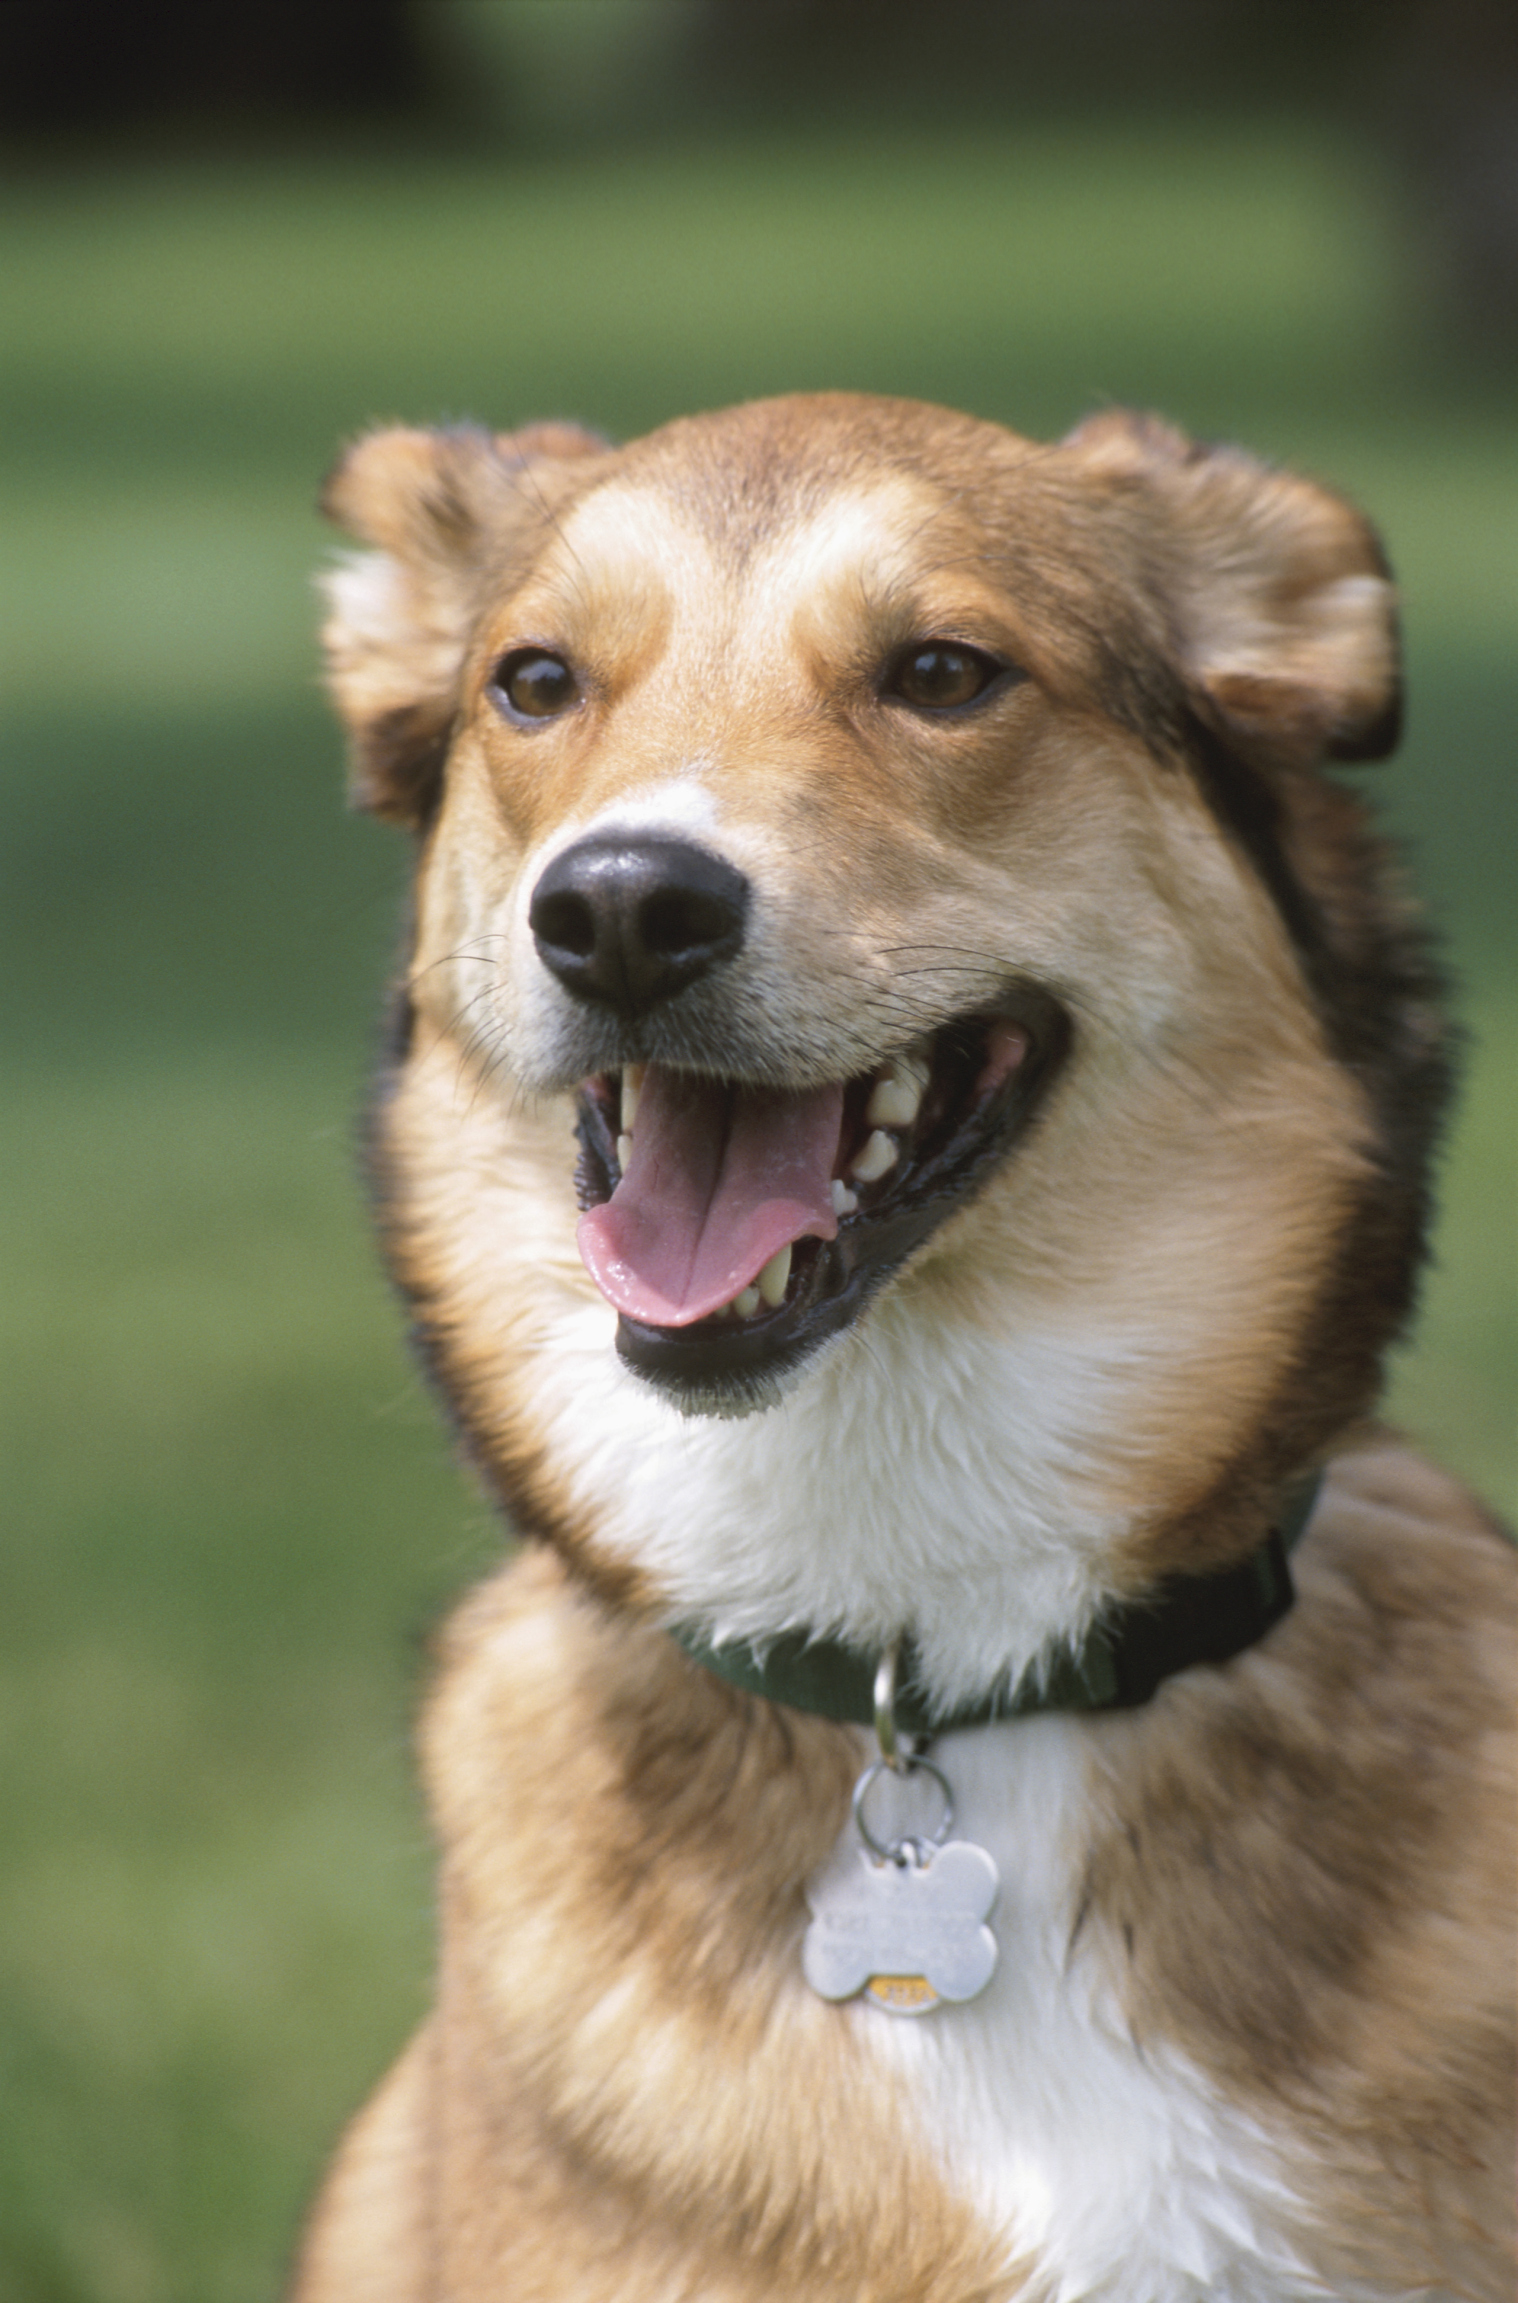
\includegraphics[width=\columnwidth]{fig/dog3-collar.jpg}
    \caption{alpha}
  \end{subfigure}
  \hfill
  \begin{subfigure}{0.2\columnwidth}
    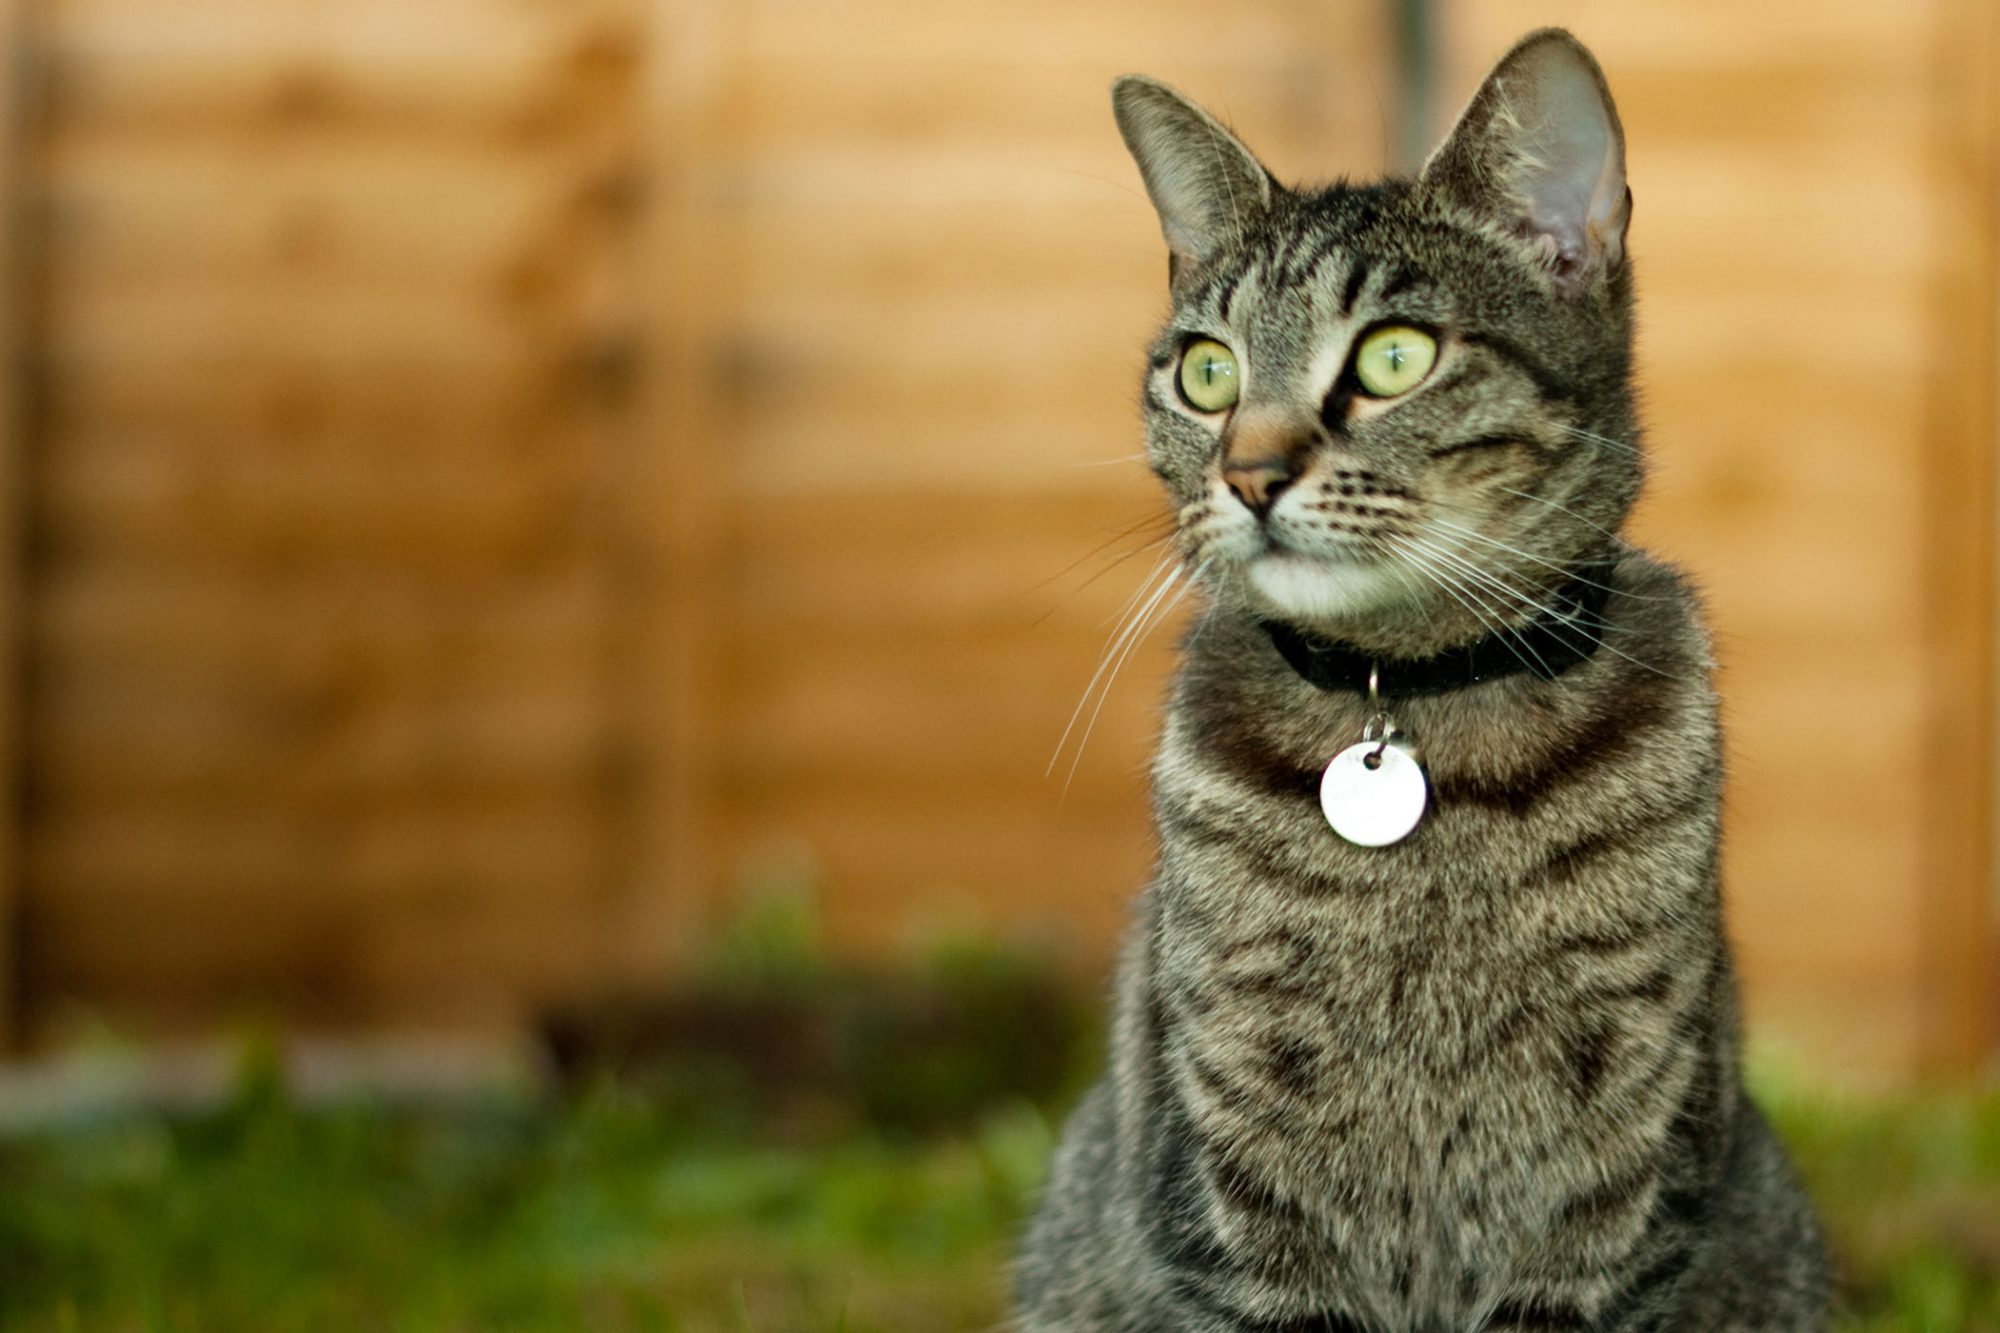
\includegraphics[width=\columnwidth]{fig/cat-collar.jpeg}
    \caption{alpha}
  \end{subfigure}
  \hfill
  \begin{subfigure}{0.2\columnwidth}
    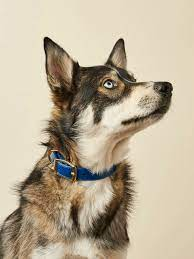
\includegraphics[width=\columnwidth]{fig/dog2-collar.jpeg}
    \caption{alpha}
  \end{subfigure}
  \hfill
  \begin{subfigure}{0.2\columnwidth}
    
\includegraphics[width=\columnwidth]{fig/cat2-collar.jpeg}
    \caption{alpha}
  \end{subfigure}
  \caption{Generalizing examples of alpha}
\end{figure}


  \pause

  \begin{exercise}
    \begin{enumerate}
      \item What does \enquote{alpha} mean?
    \end{enumerate}
  \end{exercise}
\end{frame}

\begin{frame}\label{vtcon}
  \begin{frame}
  \begin{figure}
    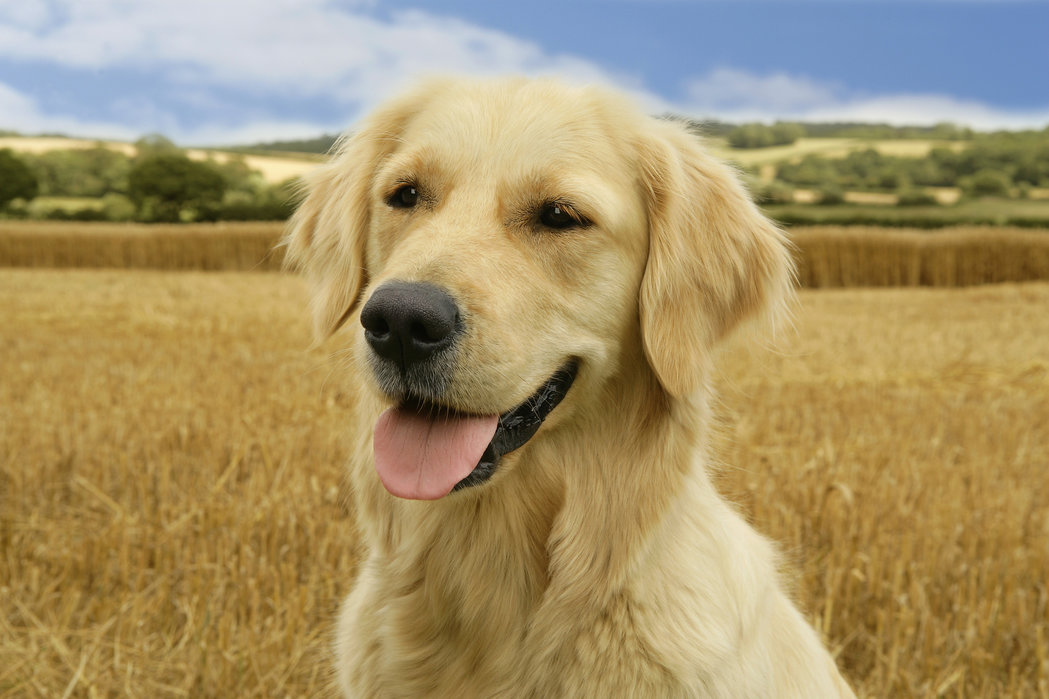
\includegraphics[height=0.8\textheight]{fig/golden-retriever.jpg}
    \caption{Example of \emph{not} alpha}
  \end{figure}
\end{frame}

\begin{frame}
  \begin{figure}
    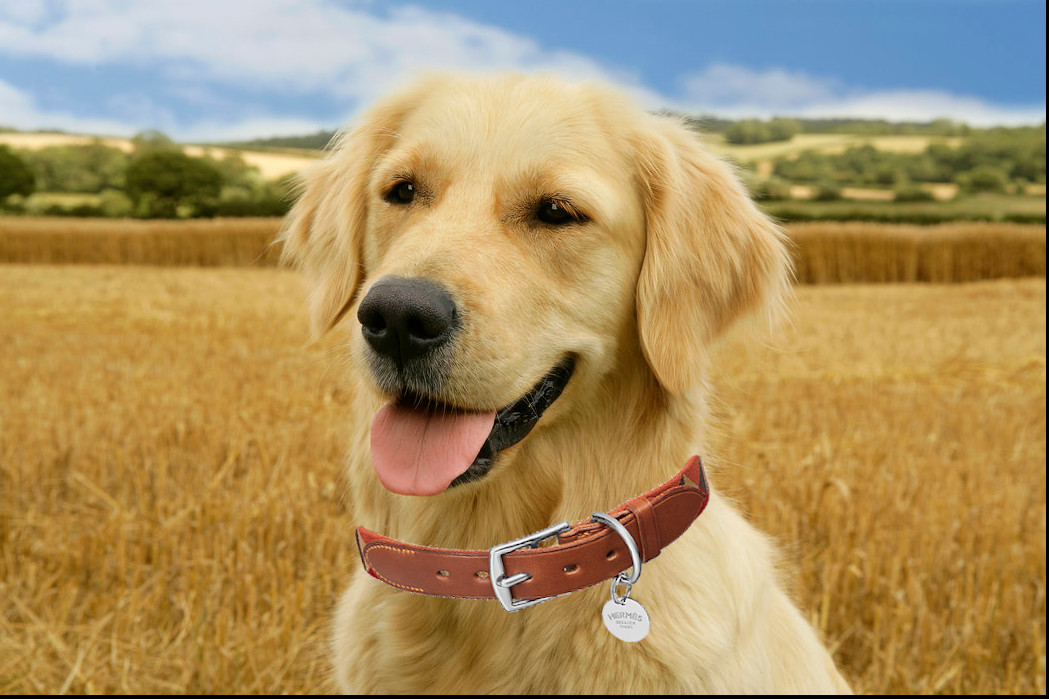
\includegraphics[height=0.8\textheight]{fig/golden-retriever-collar.jpg}
    \caption{Example of alpha}
  \end{figure}
\end{frame}


\end{frame}

\begin{frame}\label{vtgen}
  \begin{figure}
  \begin{subfigure}{0.2\columnwidth}
    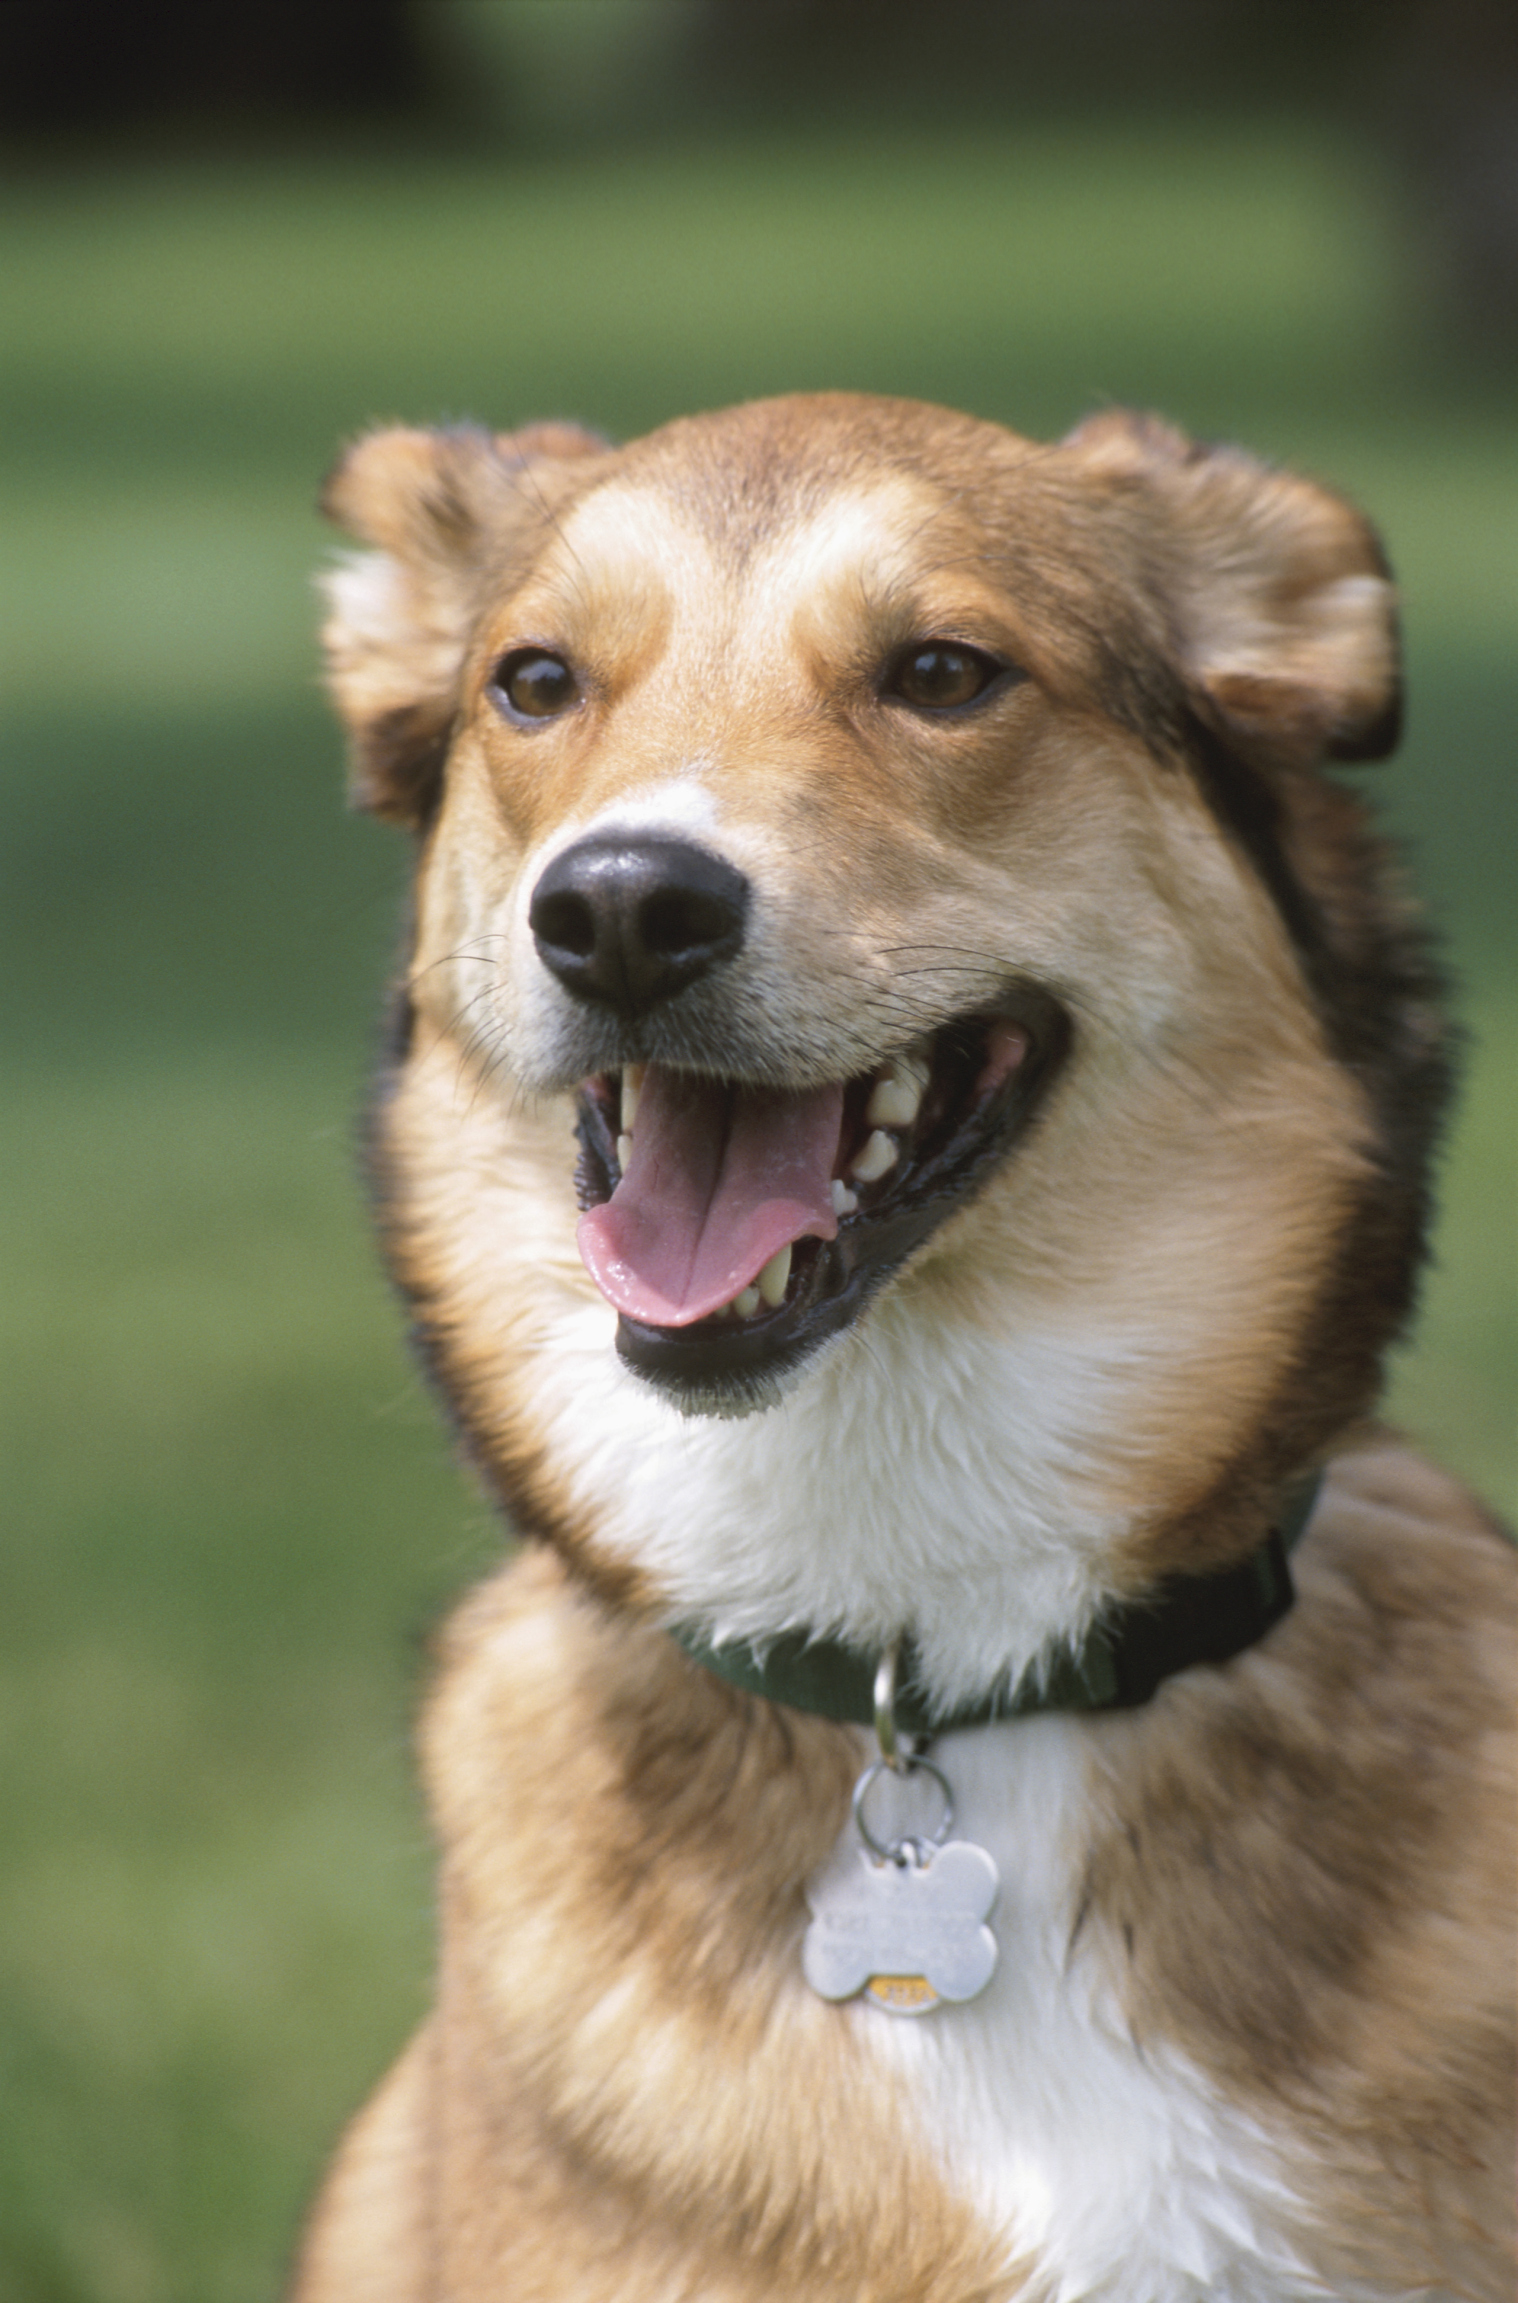
\includegraphics[width=\columnwidth]{fig/dog3-collar.jpg}
    \caption{alpha}
  \end{subfigure}
  \hfill
  \begin{subfigure}{0.2\columnwidth}
    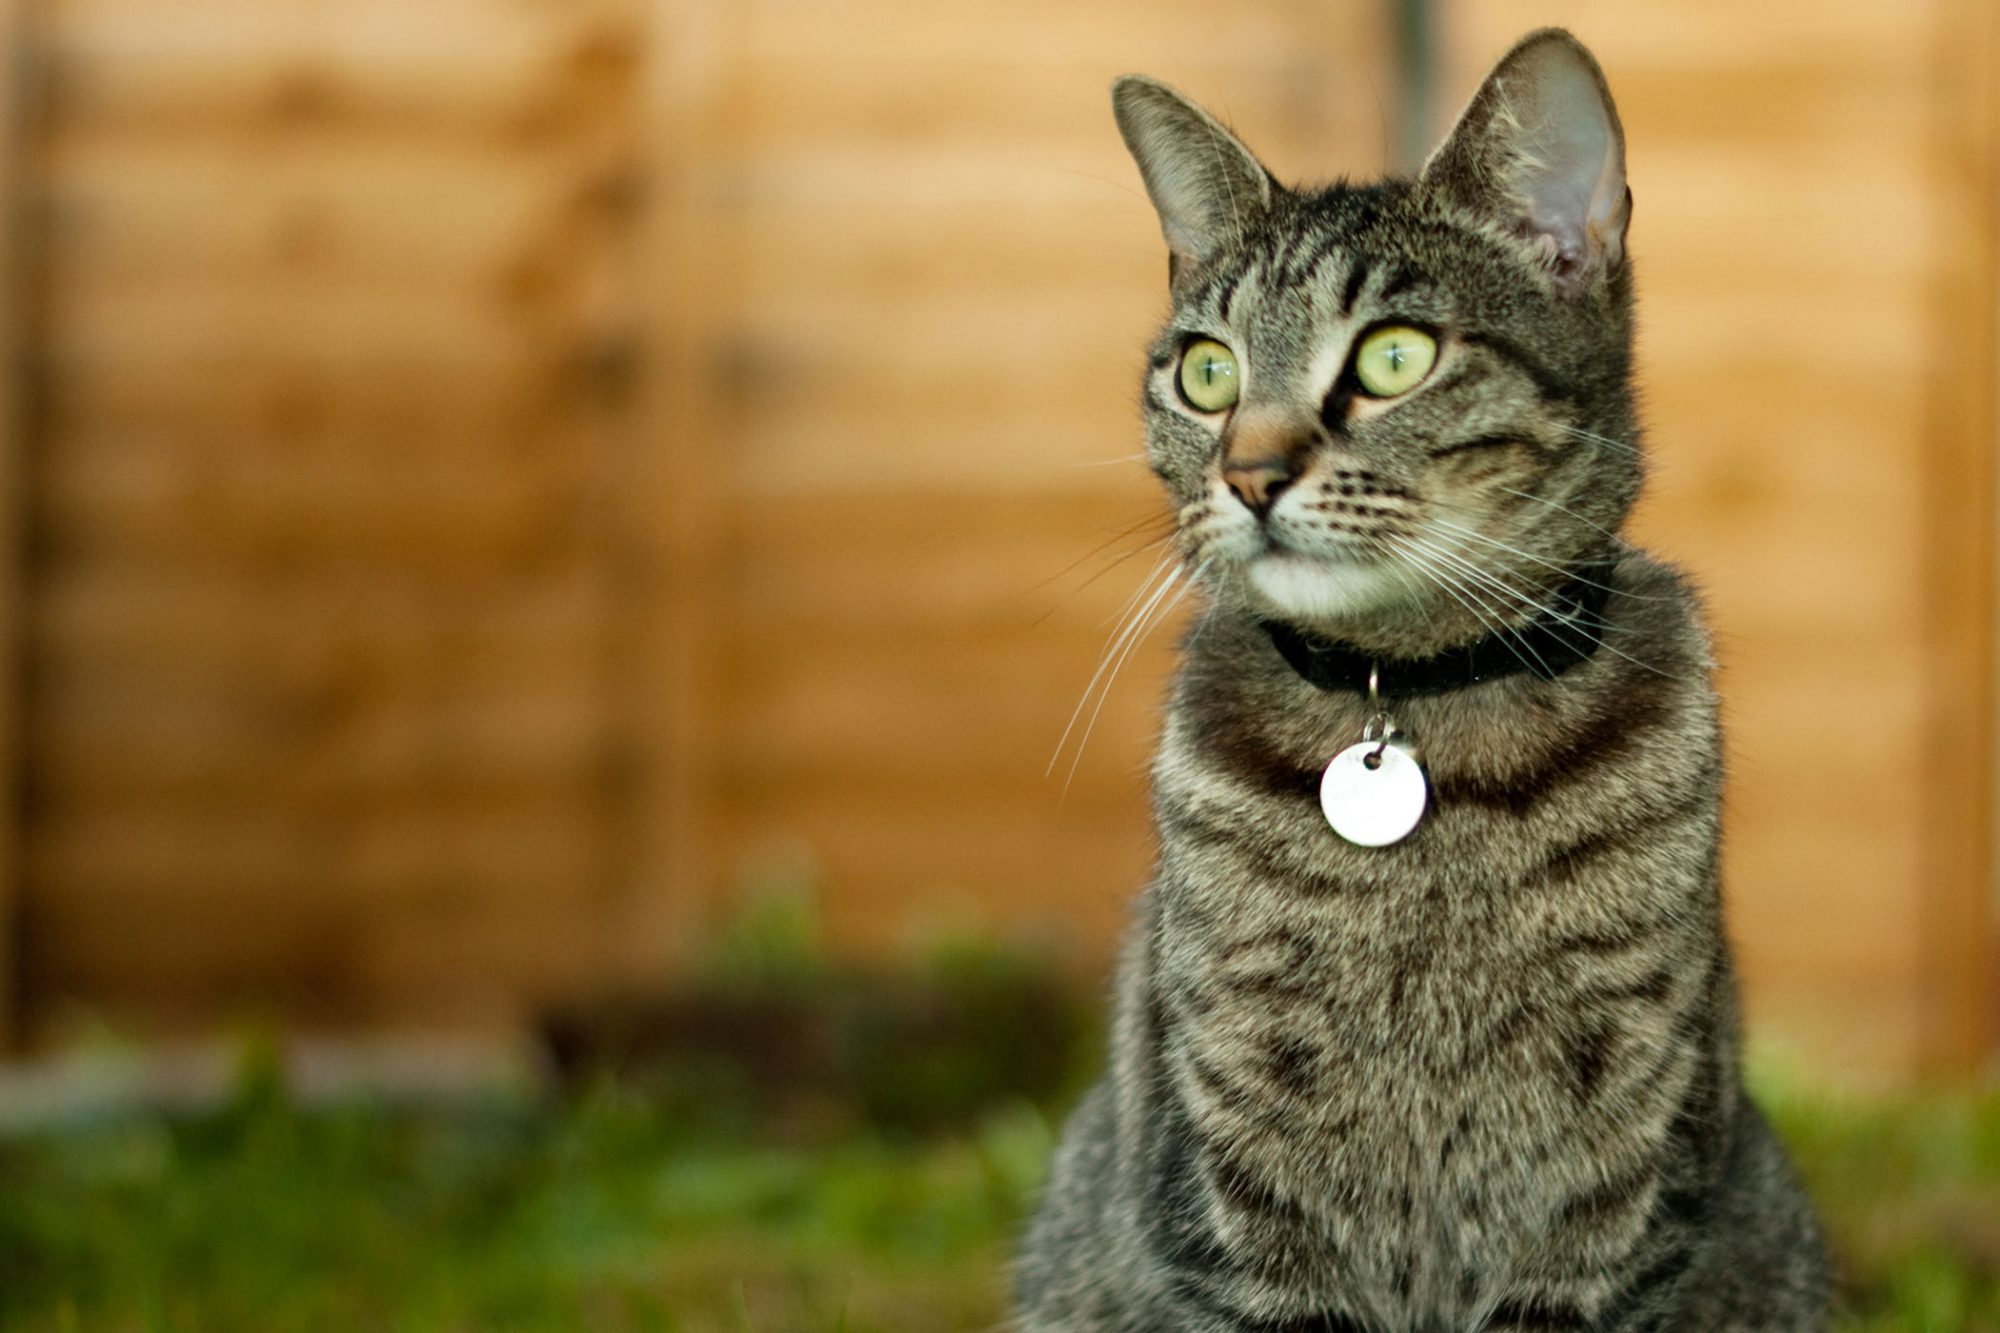
\includegraphics[width=\columnwidth]{fig/cat-collar.jpeg}
    \caption{alpha}
  \end{subfigure}
  \hfill
  \begin{subfigure}{0.2\columnwidth}
    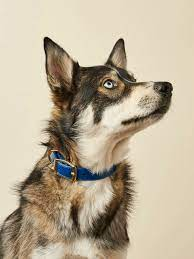
\includegraphics[width=\columnwidth]{fig/dog2-collar.jpeg}
    \caption{alpha}
  \end{subfigure}
  \hfill
  \begin{subfigure}{0.2\columnwidth}
    
\includegraphics[width=\columnwidth]{fig/cat2-collar.jpeg}
    \caption{alpha}
  \end{subfigure}
  \caption{Generalizing examples of alpha}
\end{figure}

\end{frame}

\begin{frame}
  \begin{question}[Again]
    \begin{enumerate}
      \item What does \enquote{alpha} mean?
    \end{enumerate}
  \end{question}
\end{frame}

\begin{frame}
  \begin{remark}
    \begin{itemize}
      \item Finally I gave you the \emph{contrast}.
      \item You already had the \emph{generalization}, but as \emph{induction}.
    \end{itemize}
  \end{remark}
\end{frame}

\begin{frame}
  \begin{frame}
  \begin{figure}
    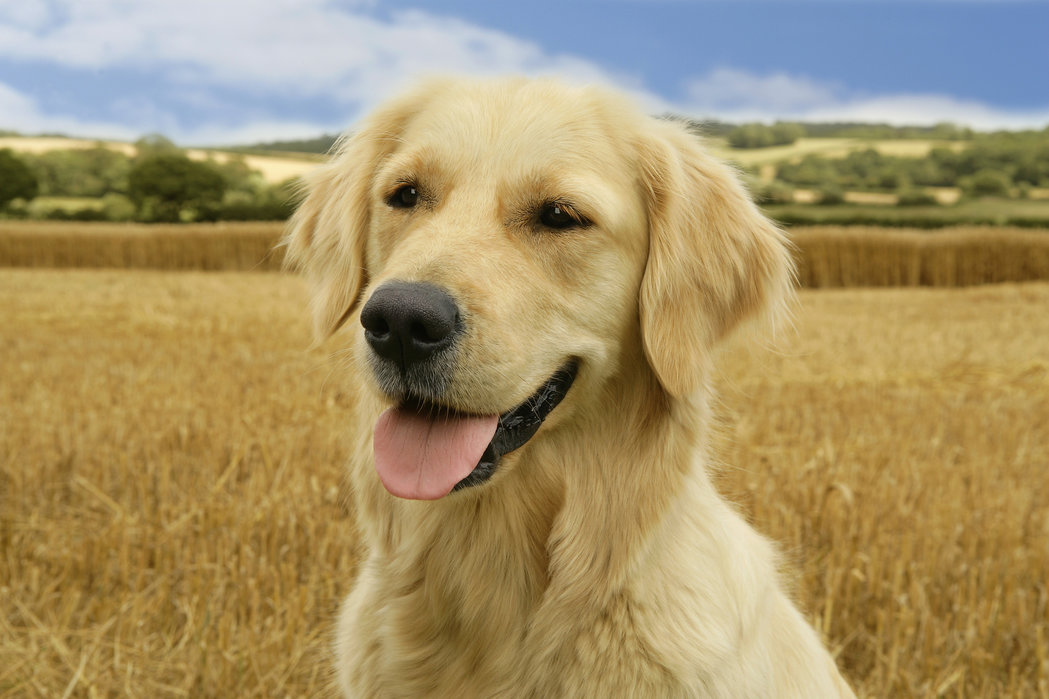
\includegraphics[height=0.8\textheight]{fig/golden-retriever.jpg}
    \caption{Example of \emph{not} alpha}
  \end{figure}
\end{frame}

\begin{frame}
  \begin{figure}
    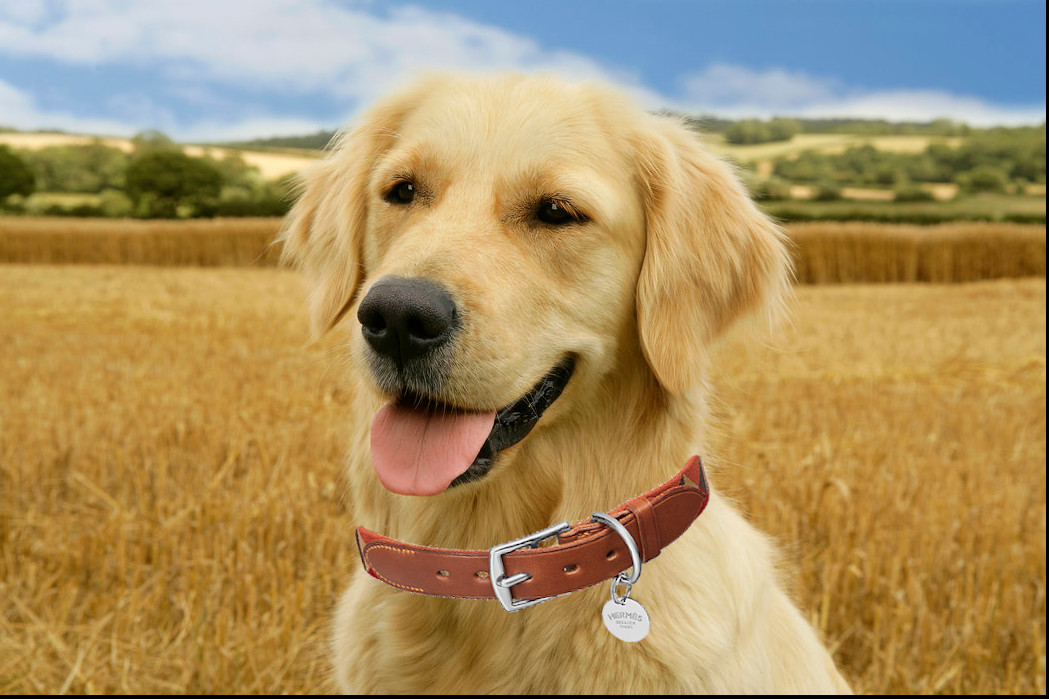
\includegraphics[height=0.8\textheight]{fig/golden-retriever-collar.jpg}
    \caption{Example of alpha}
  \end{figure}
\end{frame}


  \begin{figure}
  \begin{subfigure}{0.2\columnwidth}
    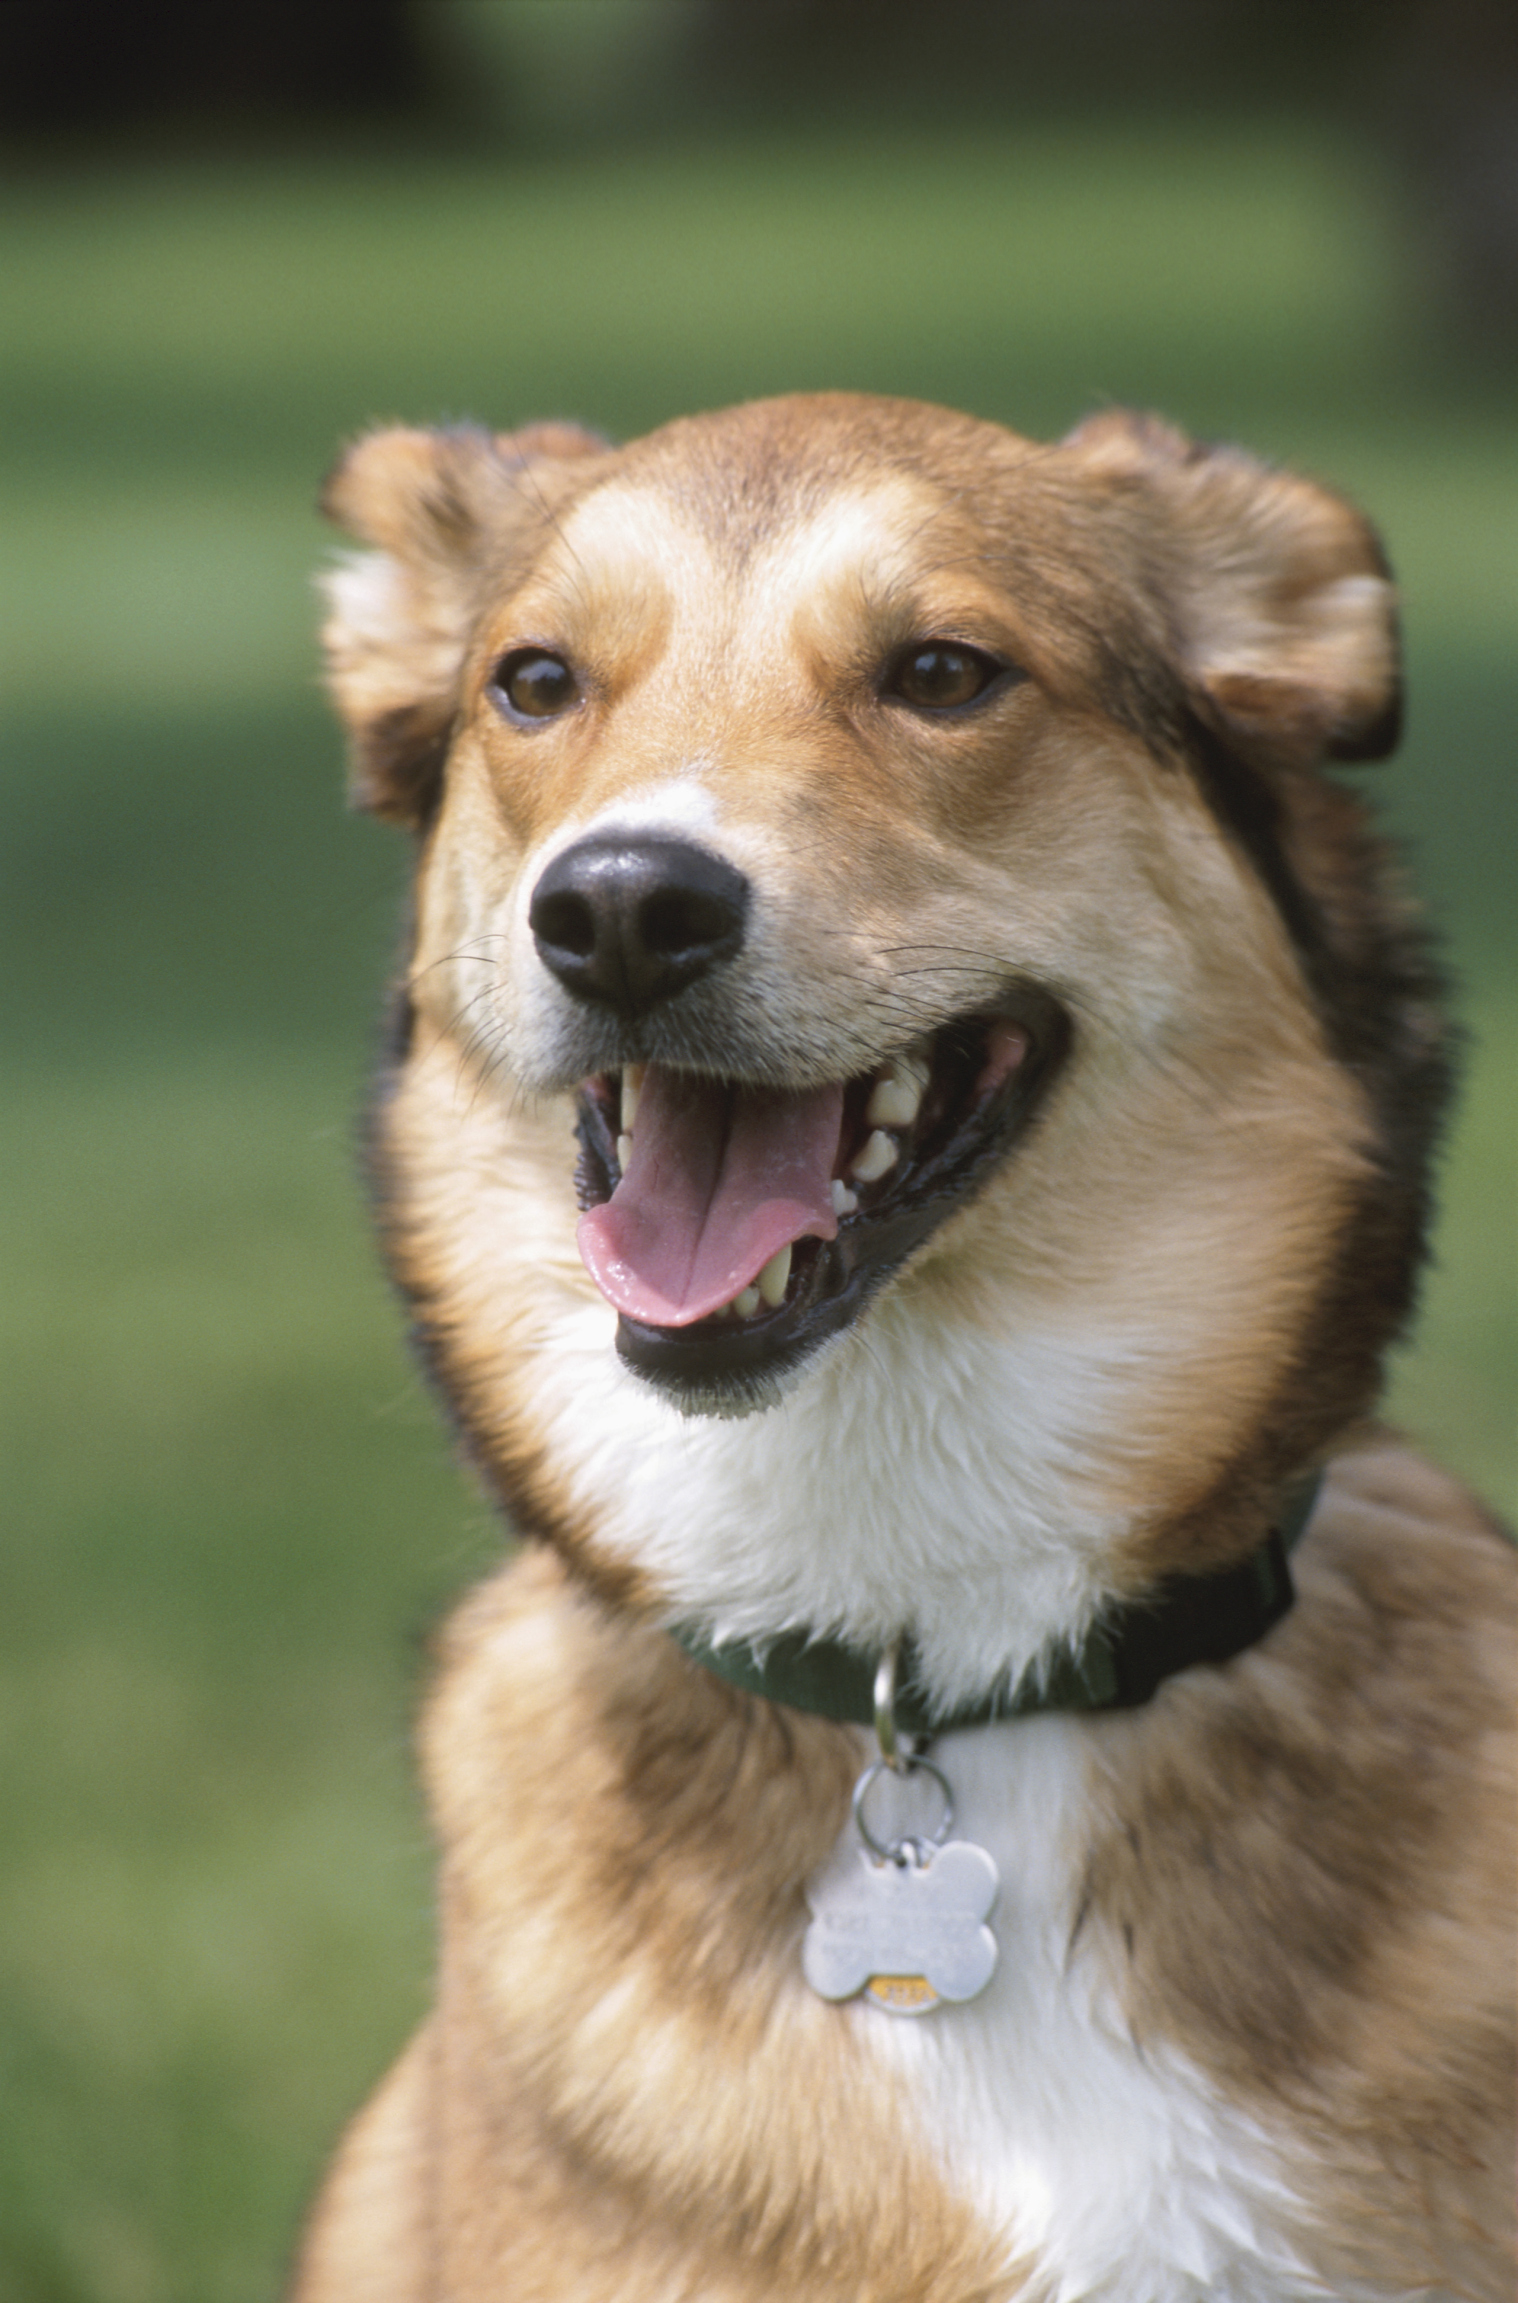
\includegraphics[width=\columnwidth]{fig/dog3-collar.jpg}
    \caption{alpha}
  \end{subfigure}
  \hfill
  \begin{subfigure}{0.2\columnwidth}
    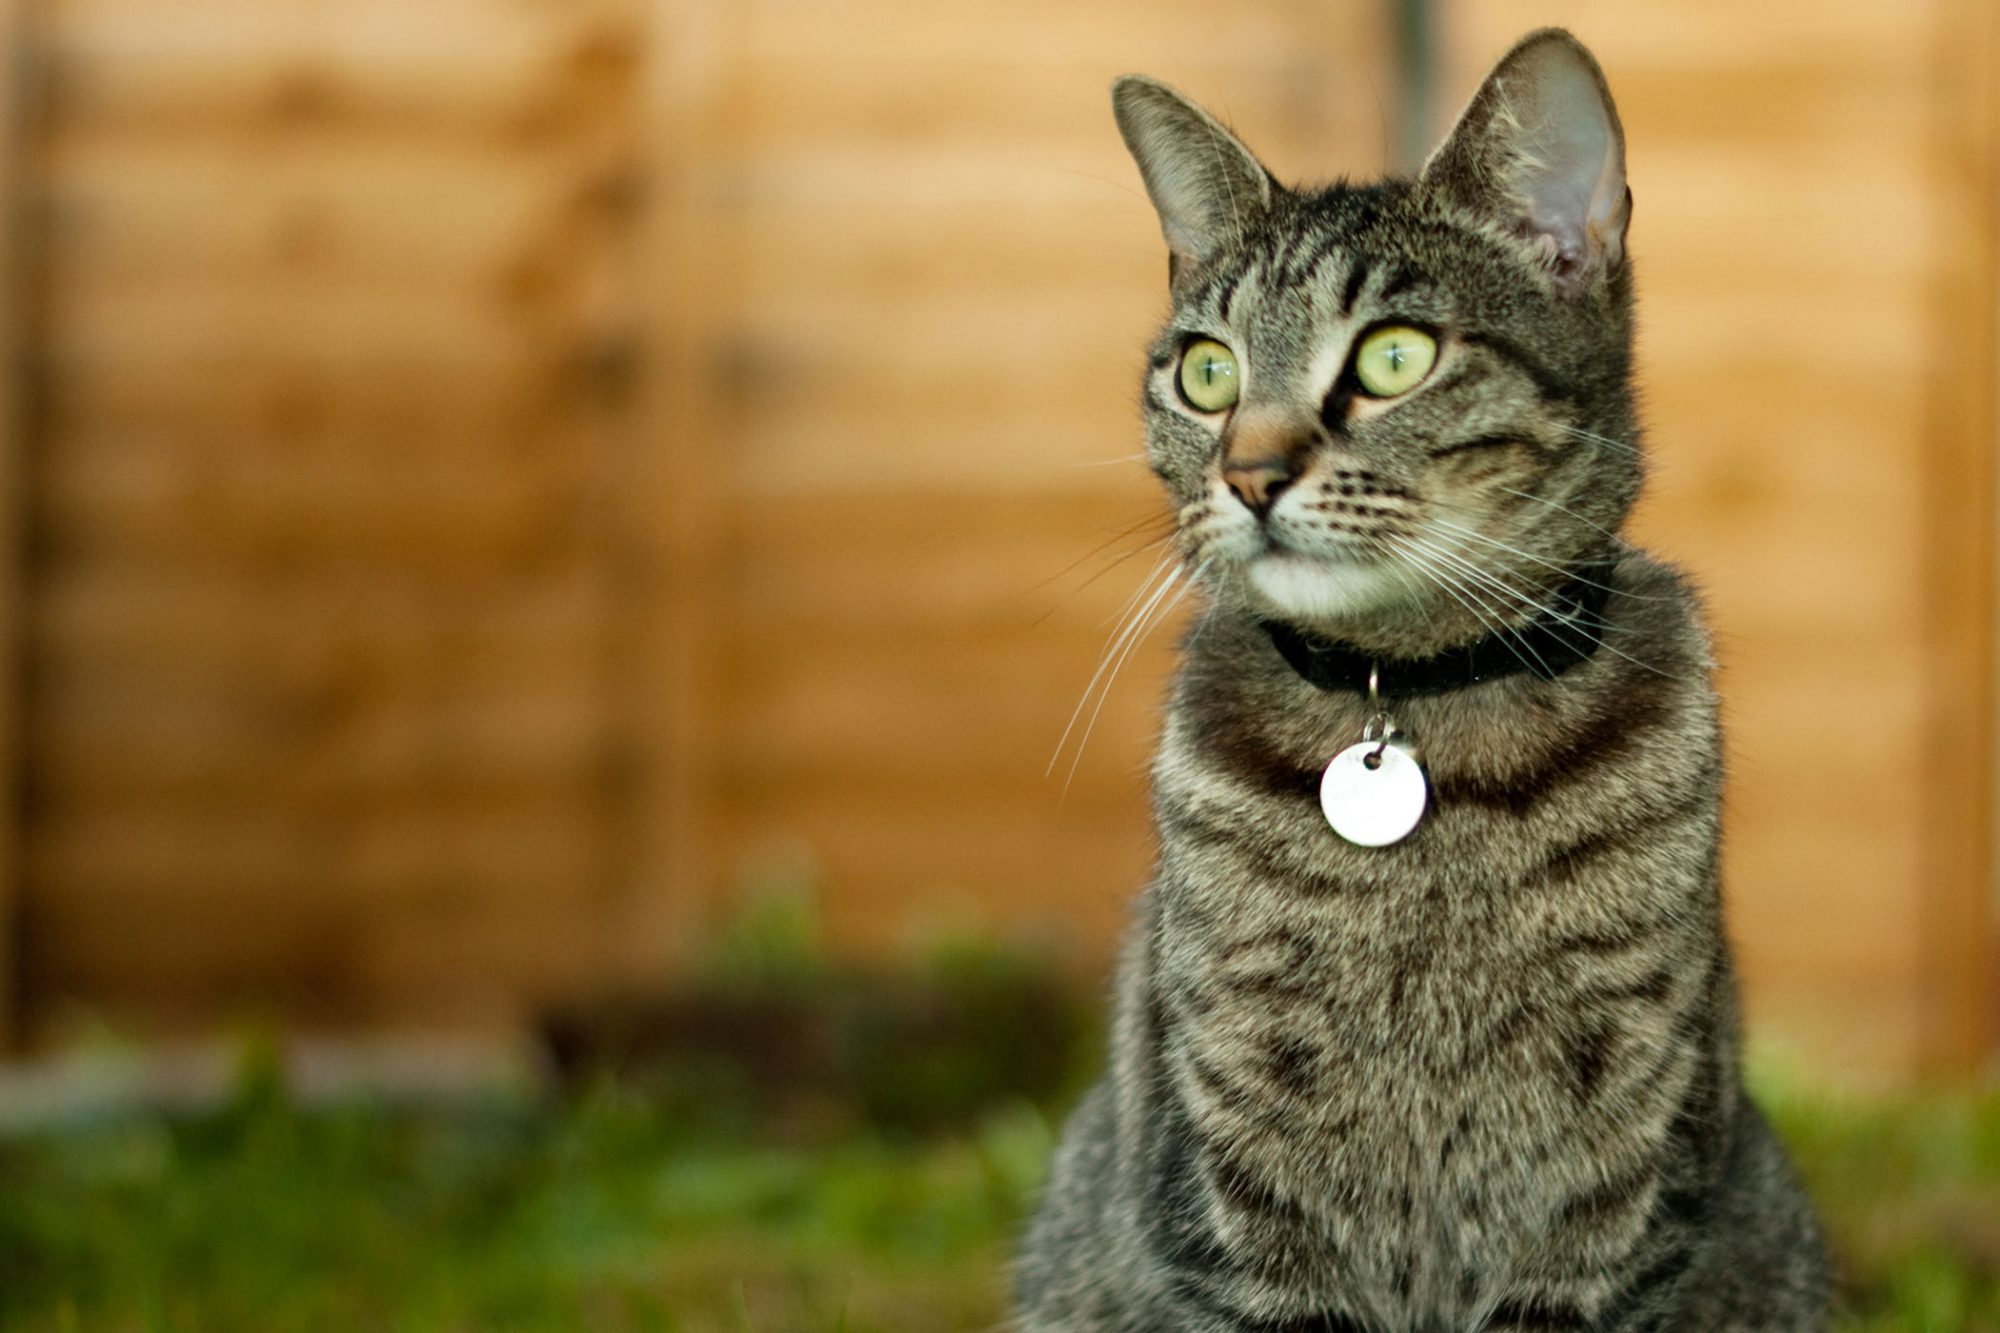
\includegraphics[width=\columnwidth]{fig/cat-collar.jpeg}
    \caption{alpha}
  \end{subfigure}
  \hfill
  \begin{subfigure}{0.2\columnwidth}
    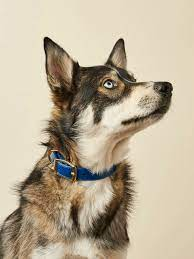
\includegraphics[width=\columnwidth]{fig/dog2-collar.jpeg}
    \caption{alpha}
  \end{subfigure}
  \hfill
  \begin{subfigure}{0.2\columnwidth}
    
\includegraphics[width=\columnwidth]{fig/cat2-collar.jpeg}
    \caption{alpha}
  \end{subfigure}
  \caption{Generalizing examples of alpha}
\end{figure}

\end{frame}

\subsection{Patterns of variation}

\begin{frame}\label<1>{vtsummary}
  \begin{figure}
    \begin{subfigure}{0.3\columnwidth}
      \centering
      \includegraphics{fig/contrast-color.tikz}
      \caption{Contrast}
    \end{subfigure}
    \hfill
    \begin{subfigure}{0.3\columnwidth}
      \centering
      \includegraphics{fig/generalization-color.tikz}
      \caption{Generalization}
    \end{subfigure}
    \hfill
    \begin{subfigure}{0.3\columnwidth}
      \centering
      \includegraphics{fig/fusion-color.tikz}
      \caption{Fusion}
    \end{subfigure}
    \caption{%
      Illustrating the patterns of variation for aspects color and shape.
    }
  \end{figure}

  \begin{onlyenv}<1>
    \begin{example}
      \begin{itemize}
        \item Critical aspect: colour.
        \item Critical feature: blue.
        \item Non-critical feature: green.
        \item Non-critical aspect: shape.
        \item Non-critical features: circle, square.
      \end{itemize}
    \end{example}
  \end{onlyenv}
  \begin{onlyenv}<2>
    \begin{remark}
      \begin{itemize}
        \item There are other aspects too, \emph{unintentionally}.
        \item Another aspect in this figure is order: the circle is always 
          \enquote{first} (to the right).
      \end{itemize}
    \end{remark}
  \end{onlyenv}
\end{frame}

\begin{frame}
  \begin{remark}
    \begin{itemize}
      \item They can appear out of order.
      \item The important thing is that the learner must juxtapose them!
      \item Thus contrast first is likely more successful.
    \end{itemize}
  \end{remark}
\end{frame}

\section{Applied to programming}

\subsection{Scope of identifiers in Python again}

\begin{frame}[fragile]\label{vtprogid}
  \begin{example}[Situation from Ch 2]
    \lstexample{examples/greet.py}
  \end{example}

  \begin{block}{Output}
    \runexample{examples/greet.py}
  \end{block}
\end{frame}

\begin{frame}[fragile]\label{vtprogidcon}
  \begin{example}[Contrast identifiers in different scopes]
    \lstexample[highlightlines=5-7]{examples/scope-contrast.py}
  \end{example}

  \begin{block}{Output}
    \runexample{examples/scope-contrast.py}
  \end{block}
\end{frame}

\begin{frame}[fragile]
  \begin{example}[Contrast identifiers in different scopes]
    \lstexample[highlightlines=5]{examples/scope-contrast-more.py}
  \end{example}

  \begin{block}{Output}
    \runexample{examples/scope-contrast-more.py}
  \end{block}
\end{frame}

\subsection{Order or arguments in Python again}

\begin{frame}[fragile]\label{vtprogord}
  \begin{example}[From Ch 2 again]
    \lstexample{examples/greet.py}
  \end{example}

  \begin{block}{Output}
    \runexample{examples/greet.py}
  \end{block}
\end{frame}

\begin{frame}[fragile]\label{vtprogordcon}
  \begin{example}[Constrast argument order]
    \lstexample[highlightlines={1,7}]{examples/order-contrast.py}
  \end{example}

  \begin{block}{Output}
    \runexample{examples/order-contrast.py}
  \end{block}
\end{frame}


\section{Some experiments}

\begin{frame}\label{vtphysics}
  \begin{example}[Physics {\cite[p.~58]{NecessaryConditionsOfLearning}}]
    \begin{enumerate}
      \item Students were introduced to modern physics.
      \item Students were introduced to modern physics, contrasted with what we 
        believed before.
    \end{enumerate}
  \end{example}
\end{frame}

\begin{frame}\label{vtunknown}
  \begin{example}[Using the known to prepare for unknown 
    {\cite[p.~68]{NecessaryConditionsOfLearning}}]
    \begin{itemize}
      \item Kids were to hit a target by throwing a shuttlecock (badminton 
        \enquote{ball}).
    \end{itemize}
    \begin{enumerate}
      \item Practicing from the same position as testing.
      \item Practicing from several positions, except the testing position.
    \end{enumerate}
  \end{example}
\end{frame}

\section{Grouping}

\begin{frame}\label<1>{vtgrouping}
  \begin{example}[Grouping on tones or sound 
    {\cite[p.~63]{NecessaryConditionsOfLearning}}]
    \begin{onlyenv}<2>
      \begin{itemize}
        \item Grouping can be done by similarity (induction) or differences 
          (contrast).
        \item Experiment teaching tonal language (\eg Cantonese) to speakers of 
          non-tonal languages (\eg Swedish).
      \end{itemize}
    \end{onlyenv}
  \end{example}

  \begin{figure}
    \only<1>{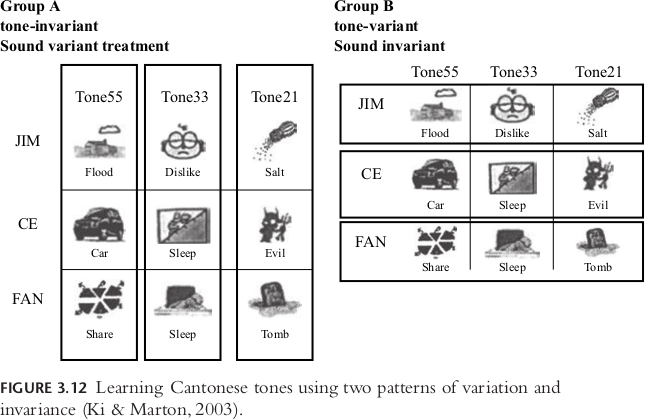
\includegraphics[height=0.8\textheight]{fig/group-tone-sound.png}}
    \only<2>{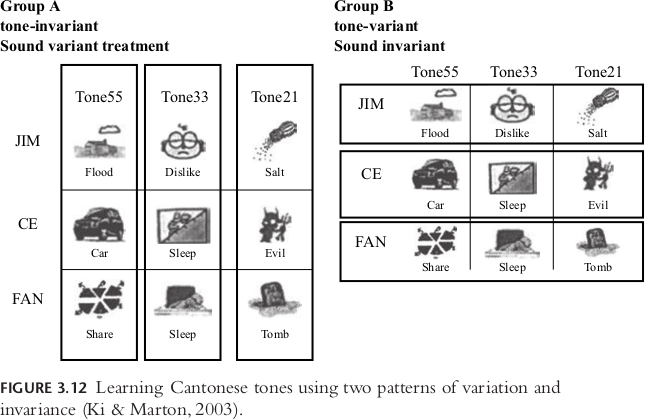
\includegraphics[height=0.5\textheight]{fig/group-tone-sound.png}}
  \end{figure}
\end{frame}

\subsection{Grouping in programming}

\begin{frame}\label<2>{vtgroupprog}
  \begin{example}[Iterations]
    \begin{itemize}
      \item We usually teach \mintinline{python}{for}, 
        \mintinline{python}{while} and recursion separately.
      \item \mintinline{python}{for}: here are examples (problems) suitable for 
        the \mintinline{python}{for} construction.
      \item \mintinline{python}{while}: here are examples (problems) suitable 
        while the \mintinline{python}{while} construction.
      \item recursion: we save this for the advanced course.
    \end{itemize}
  \end{example}

  \pause

  \begin{remark}
    \begin{itemize}
      \item Arguably, we should treat these \emph{three} at the same time.
      \item We must provide contrast between the problems suitable for the 
        different types of iterations.
      \item We'll return to this.
    \end{itemize}
  \end{remark}
\end{frame}

\section{Reflection}

\begin{frame}
  \begin{question}
    \begin{itemize}
      \item So how did we do in these slides?
    \end{itemize}
  \end{question}
\end{frame}

\begin{frame}
  \begin{figure}
    \begin{subfigure}{0.3\columnwidth}
      \includeslide[width=\columnwidth]{vtind}
      \caption{Induction}
    \end{subfigure}
    \begin{subfigure}{0.6\columnwidth}
      \includeslide[width=0.5\columnwidth]{vtcon}
      \hfill
      \includeslide[width=0.5\columnwidth]{vtgen}
      \caption{Contrast followed by generalization}
    \end{subfigure}
    \caption{Induction \emph{contrasted} to contrast-generalization.}
  \end{figure}
\end{frame}

\begin{frame}
  \begin{figure}
    \begin{subfigure}{0.3\columnwidth}
      \includeslide[width=\columnwidth]{vtsummary}
      \caption{Summary}
    \end{subfigure}
    \begin{subfigure}{0.6\columnwidth}
      \includeslide[width=0.5\columnwidth]{vtprogid}
      \includeslide[width=0.5\columnwidth]{vtprogidcon}
      \caption{Contrast identifiers}
    \end{subfigure}
    \begin{subfigure}{0.6\columnwidth}
      \includeslide[width=0.5\columnwidth]{vtprogord}
      \includeslide[width=0.5\columnwidth]{vtprogordcon}
      \caption{Contrast order}
    \end{subfigure}
    \caption{\emph{Generalizing} the contrast-generalization pattern.}
  \end{figure}
\end{frame}

\begin{frame}
  \begin{figure}
    \begin{subfigure}{0.3\columnwidth}
      \includeslide[width=\columnwidth]{vtphysics}
      \caption{Physics}
    \end{subfigure}
    \begin{subfigure}{0.3\columnwidth}
      \includeslide[width=\columnwidth]{vtunknown}
      \caption{Known to unknown}
    \end{subfigure}
    \caption{\emph{Generalizing} further, learner generates patterns.}
  \end{figure}
\end{frame}

\begin{frame}
  \begin{figure}
    \begin{subfigure}{0.3\columnwidth}
      \includeslide[width=\columnwidth]{vtprogidcon}
      \caption{Identifier}
    \end{subfigure}
    \begin{subfigure}{0.3\columnwidth}
      \includeslide[width=\columnwidth]{vtprogordcon}
      \caption{Order}
    \end{subfigure}
    \newline
    \begin{subfigure}{0.3\columnwidth}
      \includeslide[width=\columnwidth]{vtgrouping}
      \caption{Tones--sounds}
    \end{subfigure}
    \begin{subfigure}{0.3\columnwidth}
      \includeslide[width=\columnwidth]{vtgroupprog}
      \caption{Iterations}
    \end{subfigure}
    \caption{\emph{Contrasting} how to contrast by introducing grouping,
      \emph{generalizing} by iterations example.}
  \end{figure}
\end{frame}

% slides on grouping
